\chapter{A Tight Bound on Grids of Size $\geq$ 5}

\section{Introduction and Definitions}
Let the ordered tuple $(a,b,c)$ represent the $a \times b \times c$ grid $G$ where $a \geq b \geq c$. We refer to $c$ as the \emph{thickness} of $G$. For example, the tuple $(5,3,3)$ represents a $5 \times 3 \times 3$ grid of thickness 3. We refer to a tuple as \emph{divisible}, or a \emph{divisibility case}, if and only if $ab+bc+ca \equiv 0 \pmod 3$. If a tuple is divisible and percolates at the lower bound, we refer to it as \emph{perfect}. Observe that the divisibility cases are precisely those grids with integral lower bounds. The divisibility cases of thicknesses belonging to the three residue classes modulo 3 are illustrated in \{Figure something\}.

In the following lemmas, we use the notation $(a,b,c)+(x,y,z) = (a+x, b+y, c+z)$ to represent respective increases of $x$, $y$, and $z$ to the side lengths $a$, $b$, and $c$ of $G$. We note the following: 
\begin{rem}
\label{rem:recursion_pieces}
By applying the recursion, $(a,b,c)+(x,y,z)$ percolates at the lower bound when either:
\begin{enumerate}
\item $(a,b,c), (a,y,z), (x,b,z), (x,y,c)$ all percolate at the lower bound; or
\item $(x,y,z), (x,b,c), (a,y,c), (a,b,z)$ all percolate at the lower bound.
\end{enumerate}
\end{rem}

We shall call a thickness \emph{complete} if it can be shown that all divisibility cases in that thickness are perfect. In this section, we demonstrate that thickness 5, thickness 6 and thickness 7 are all complete. As these belong to the residue classes 2, 0, and 1 modulo 3, respectively, we then use a recursive construction to show that all larger grids are also complete. 

\section{Completeness of Thickness 5}
We show that all divisibility cases for grids of thickness 5 admit perfect lethal sets. Observe that divisibility cases for thickness 5 consist of grids of the form $(x,y,5)$ where $x$ and $y$ are in residue classes $\{0,2,3,5\}$ modulo 6 (see Table \ref{fig:thickness_5_cases}). We separate these divisibility cases into the following four categories and show that each category is complete:

\begin{enumerate}
\item $(x,5,5)$ for $x \in \{2,5\} \pmod 6$;
\item $(x,6,5)$ for $x \in \{0,3\} \pmod 6$;
\item $(x,y,5)$ for $x,y \in \{0,2,3,5\} \pmod 6$ and $x \not\equiv y$;
\item $(x,y,5)$ for $x,y \in \{0,2,3,5\} \pmod 6$ and $x \equiv y$;
\end{enumerate}

\begin{table}[]
\centering
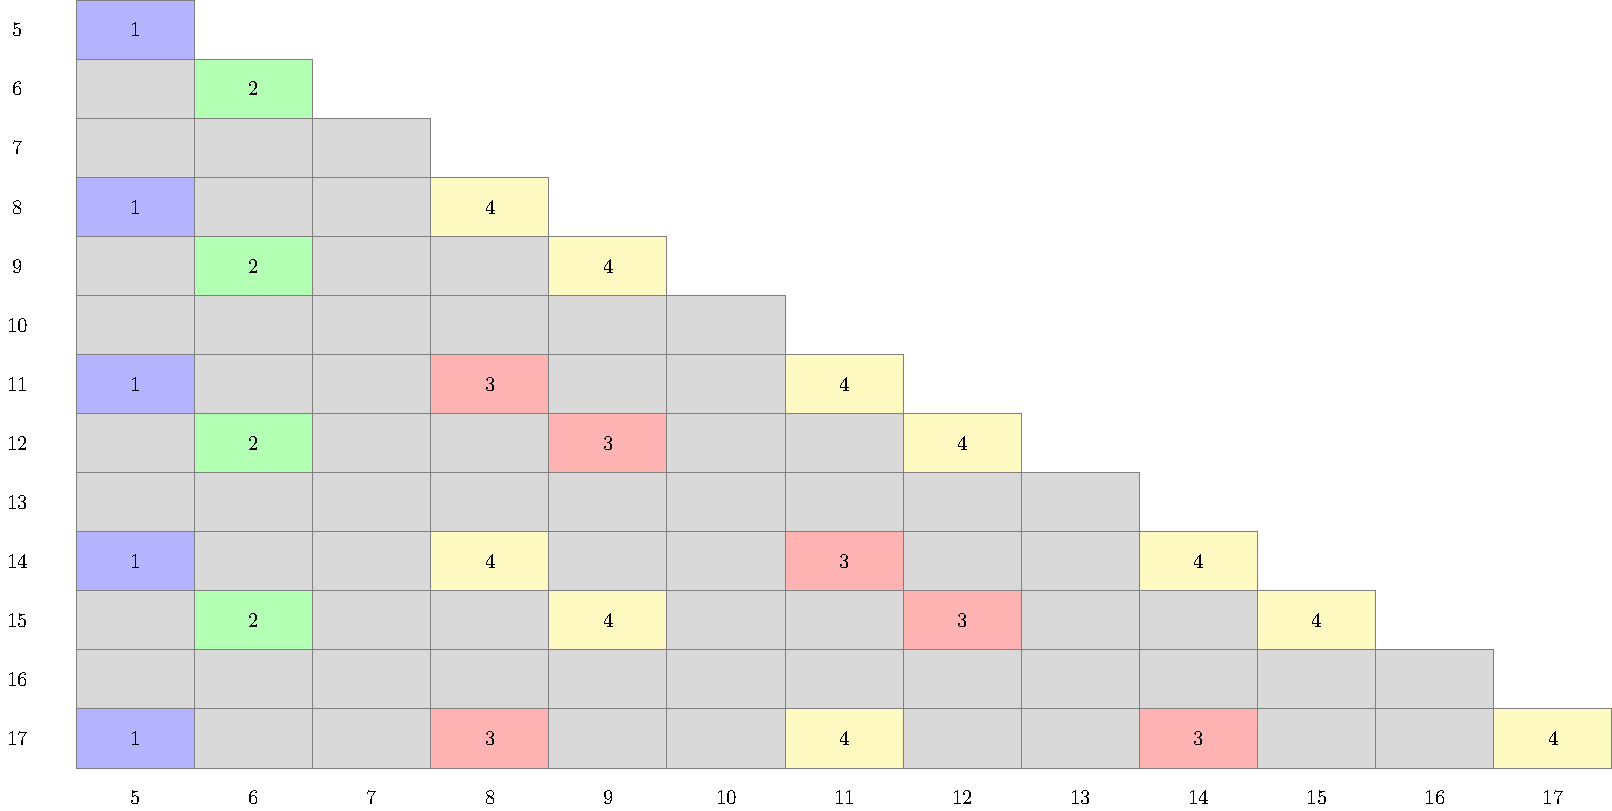
\includegraphics[width=\textwidth]{tables/4/thickness_5_cases.pdf}
\caption{The four thickness 6 cases analyzed in Lemmas \ref{lem:thickness_5_case_1} (blue), \ref{lem:thickness_5_case_2} (green), \ref{lem:thickness_5_case_3} (red), and \ref{lem:thickness_5_case_4} (yellow).}
\label{fig:thickness_5_cases}
\end{table}

%Leveraging \{lemmas from earlier chapters yet to be written\}, we show that all divisibility cases in thickness 5 percolate at the lower bound. 

%NOTE: THE FOLLOWING LEMMAS HOLD ASSUMING WE HAVE A GENERAL CONSTRUCTION FOR $(2,3,3k)$ FOR ALL $k$.
\begin{lem}
\label{lem:thickness_5_case_1}
All grids of the form $(x,5,5)$ for $x \in \{2,5\} \pmod 6$ admit perfect lethal sets.
\end{lem}

\begin{proof}
Consider the construction $(5,2,2) + (a,3,3)$, for $a \equiv 0 \pmod 3$ and $a >3$. Observe that this construction obtains all grids of the form described in (1), apart from $(5,5,5)$ and $(8,5,5)$.

By Corollary \ref{cor:recursion}, we must show that the grids $(5,2,2), (5,3,3), (a,2,3), (a,3,2)$ are all perfect. We have that $(5,2,2)$ is perfect by Construction \ref{con:5x2x2} in Appendix A, and $(5,3,3)$ is given by Proposition \ref{prop:3x3xk}. Since $a >3$, Propositions \ref{prop:2x3xk_0} and \ref{prop:2x3xk_3} give $(a,2,3)$. 

By Constructions \ref{con:5x5x5} and \ref{con:8x5x5} in Appendix A, we obtain the remaining grids $(5,5,5)$ and $(8,5,5)$. We conclude that all grids of the form given in (1) are perfect.
\end{proof}

\begin{lem}
\label{lem:thickness_5_case_2}
All grids of the form $(x,6,5)$ for $x \in \{0,3\} \pmod 6$ admit perfect lethal sets.
\end{lem}

\begin{proof}
Consider the construction $(6,3,2) + (a,3,3)$, for $a \equiv 0 \pmod 3$ and $a >3$. Observe that this construction obtains all grids of the form described in (1), apart from $(6,6,5)$ and $(9,6,5)$.

By Corollary \ref{cor:recursion}, we must show that the grids $(6,3,2), (6,3,3), (a,3,3), (a,3,2)$ are all perfect. Since $a >3$, $(6,3,2)$ and $(a,3,2)$ are given by Propositions \ref{prop:2x3xk_0} and \ref{prop:2x3xk_3}. Similarly, $(6,3,3)$ and $(a,3,3)$ are given by Proposition \ref{prop:3x3xk}.

To obtain $(6,6,5)$, we consider the construction $(3,3,1)+(3,3,4)$. By Corollary \ref{cor:recursion}, we must show that $(3,3,1), (3,3,4), (3,3,4), (3,3,1)$ are all perfect. These are obtained, respectively, by Propositions \ref{prop:3x3xk} and \ref{prop:thickness_3_width_4}. Construction \ref{con:9x6x5} gives $(9,6,5)$. We conclude that all grids of the form given in (2) are perfect.
\end{proof}

\begin{lem}
\label{lem:thickness_5_case_3}
All grids of the form $(x,y,5)$ for $x,y \in \{0,2,3,5\} \pmod 6$ and $x \not\equiv y$ admit perfect lethal sets.
\end{lem}

\begin{proof}
Consider the construction $(a,b,2) + (6,6,3)$, for $a,b \in \{0,2,3,5\} \pmod 6$, $a \not\equiv b \pmod 6$, and $a,b > 2$. Observe that this construction obtains all grids of the form described in (3), apart from $(a,8,5)$ for $a \equiv 5 \pmod 6$ and $a \geq 11$.

By Corollary \ref{cor:recursion}, we must show that the grids $(a,b,2), (a,6,3), (6,b,3), (6,6,2)$ are all perfect. By Proposition \ref{prop:thickness_2_2d_family}, $(a,b,2)$ is perfect. Both $(a,6,3)$ and $(6,b,3)$ follow from Proposition \ref{prop:3x6xk}. We obtain $(6,6,2)$ from $(3,3,1)+(3,3,1)$. By Proposition \ref{prop:purina}, $(3,3,1)$ is perfect, and so by Corollary \ref{cor:recursion}, $(6,6,2)$ is perfect.

To obtain $(a,8,5)$, for $a \equiv 5 \pmod 6$ and $a \geq 17$, we consider the construction $(8,5,2) + (a,3,3)$, for $a \equiv 3 \pmod 6$ and $a>3$. By Corollary \ref{cor:recursion}, we must show that $(2,5,2)$, $(8,3,3)$, $(a,5,3)$, $(a,2,3)$ are all perfect. We obtain $(2,5,2)$ from Construction \ref{con:5x2x2} and $(8,3,3)$ from Proposition \ref{prop:3x3xk}. Since $a \equiv 3 \pmod 6$, Proposition \ref{prop:thickness_2_2d_family} gives $(a,5,3)$, and Proposition \ref{prop:2x3xk_3} gives $(a,2,3)$. 

The above construction omits the singular grid $(11,8,5)$. However, we may obtain $(11,8,5)$ from $(2,3,6)+(3,5,5)$. By Corollary \ref{cor:recursion}, we must show that $(2,3,6), (2,5,5)$, $(3,3,5), (3,5,6)$ are all perfect. We obtain $(2,5,5)$ from Construction \ref{con:5x5x2}, $(3,3,5)$ from Proposition \ref{prop:3x3xk}, and $(2,3,6)$ and $(3,5,6)$ from Proposition \ref{prop:3x6xk}. We conclude that all grids of the form given in (3) are perfect.
\end{proof}

\begin{lem}
\label{lem:thickness_5_case_4}
All grids of the form $(x,y,5)$ for $x,y \in \{0,2,3,5\} \pmod 6$ and $x \equiv y$ admit perfect lethal sets.
\end{lem}

\begin{proof}
Consider the construction $(a,b,2) + (6,3,3)$, for $a,b \in \{0,2,3,5\} \pmod 6$, $a \not\equiv b \pmod 6$, and $a,b > 2$. Observe that this construction obtains all grids of the form described in (4), apart from $(8,8,5)$.

By Corollary \ref{cor:recursion}, we must show that the grids $(a,b,2), (a,3,3), (6,b,3), (6,3,2)$ are all perfect. By Proposition \ref{prop:thickness_2_2d_family}, $(a,b,2)$ is perfect. Both $(6,3,2)$ and $(6,b,3)$ follow from Proposition \ref{prop:3x6xk}. We obtain $(a,3,3)$ from Proposition \ref{prop:3x3xk}.

To obtain $(8,8,5)$, we consider the construction $(2,2,2) + (6,6,3)$. By Corollary \ref{cor:recursion}, we must show that $(2,2,2), (2,6,6), (3,2,6), (3,6,2)$ are all perfect. We obtain $(2,2,2)$ from Construction \ref{con:2x2x2} and $(3,6,2)$ from Proposition \ref{prop:3x6xk}. The construction $(3,3,1)+(3,3,1)$ gives $(6,6,2)$. By Proposition \ref{prop:purina}, $(3,3,1)$ is perfect, and so by Corollary \ref{cor:recursion}, $(6,6,2)$ is perfect. We conclude that all grids of the form given in (3) are perfect.
\end{proof}

\begin{lem}
\label{lem:thickness_5_complete}
Thickness 5 is complete.
\end{lem}

\begin{proof}
By Lemmas \ref{lem:thickness_5_case_1}, \ref{lem:thickness_5_case_2}, \ref{lem:thickness_5_case_3}, and \ref{lem:thickness_5_case_4}, all divisibility cases for thickness 5 admit perfect lethal sets.
\end{proof}

\section{Completeness of Thickness 6}
We show that all divisibility cases for grids of thickness 6 admit perfect lethal sets. Observe that divisibility cases for thickness 6 consist of grids of the form $(x,y,6)$ where, without loss of generality, $x$ is in residue classes $\{0,3\}$ modulo 6, and $y$ is either even or odd (see Table \ref{fig:thickness_6_cases}). We separate these divisibility cases into the following four categories and show that each category is complete:

\begin{enumerate}
\item $(x,y,6)$ for $x \equiv 0 \pmod 6$ and $y \equiv 0 \pmod 2$;
\item $(x,y,6)$ for $x \equiv 3 \pmod 6$ and $y \equiv 1 \pmod 2$;
\item $(x,y,6)$ for $x \equiv 3 \pmod 6$ and $y \equiv 0 \pmod 2$;
\item $(x,y,6)$ for $x \equiv 0 \pmod 6$ and $y \equiv 1 \pmod 2$.
\end{enumerate}

%We shall show that all grids of thickness 6 can be obtained recursively from $(3n, m, 3)$, where $n,m \equiv 1 \pmod 2$ (this is that general thickness 3 construction), and one of $\{(3,3,3), (6,6,3), (6,3,3), (3,6,3)\}$. We examine each of these cases separately and show that each is complete. 

%(NOTE (to Peter and Jon): I have struggled a bit with the canonical way to describe grids. I like the tuple representation $(a,b,c)$ where WLOG $a \leq b \leq c$. However, this becomes a bit mucky in the following proofs, because $(3n,m,3)$ potentially violates this rule if $n$ is large and $m$ is small. To accommodate this, I have written ``grids of the form $(a,b,6)$, where $a \equiv 0 \pmod 6$ and $b \equiv 0 \pmod 2$, or $b \equiv 0 \pmod 6$ and $a \equiv 0 \pmod 2$," in an attempt to address the circumstance where the ordering of the tuple is flipped because $n$ is large and $m$ is small. However, I think this may just muddy the waters.)

%\begin{figure}[]
%\centering
%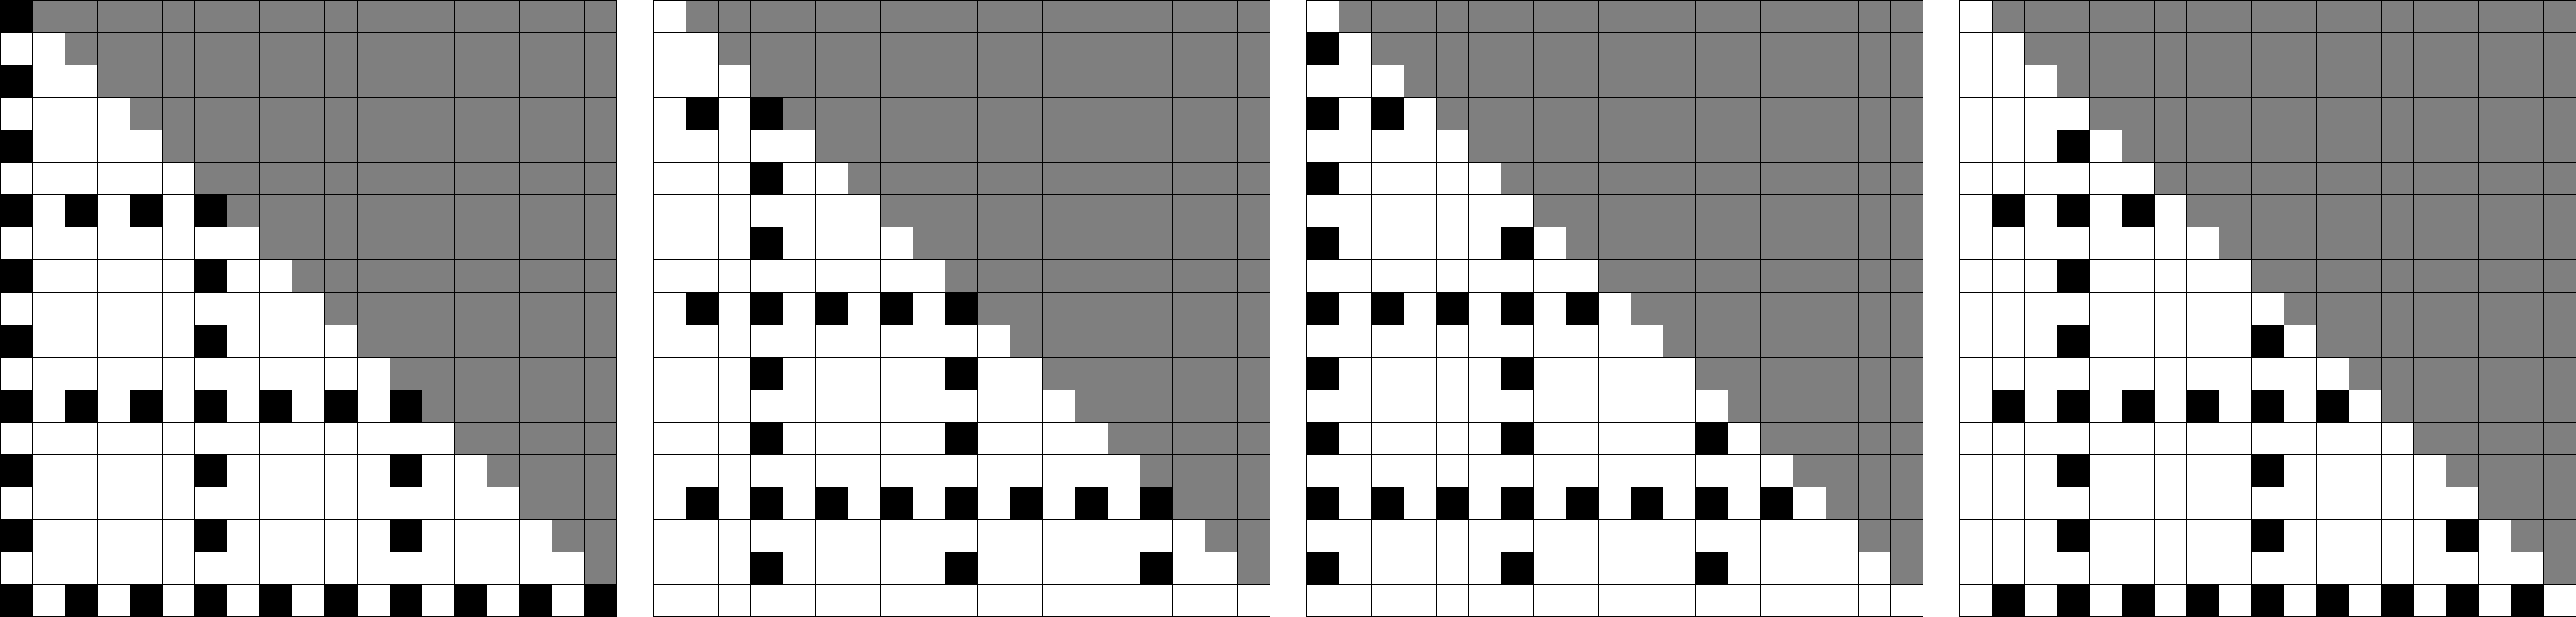
\includegraphics[width=\textwidth]{figures/4/thickness_6_case_1.pdf}
%\caption{Thickness 6 grids with perfect percolating sets as obtained in lemma \ref{lem:thickness_6_case_1} (left), and divisibility cases of thickness 6 (right).}
%\label{fig:thickness_6_case_1}
%\end{figure}

\begin{table}[]
\centering
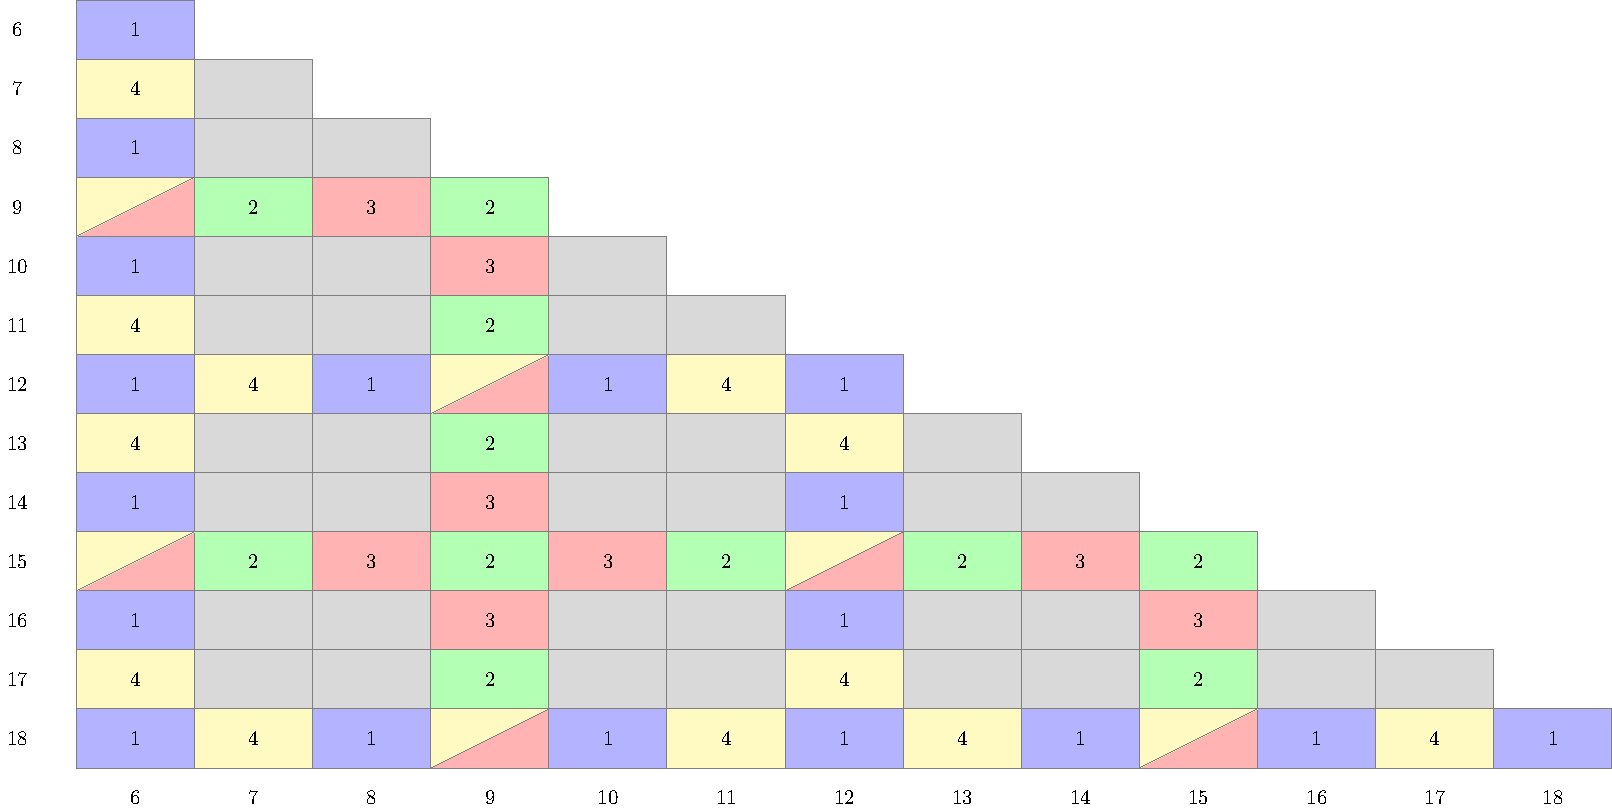
\includegraphics[width=\textwidth]{tables/4/thickness_6_cases.pdf}
\caption{The four thickness 6 cases analyzed in Lemmas \ref{lem:thickness_6_case_1} (blue), \ref{lem:thickness_6_case_2} (green), \ref{lem:thickness_6_case_3} (red), and \ref{lem:thickness_6_case_4} (yellow).}
\label{fig:thickness_6_cases}
\end{table}

\begin{lem}
\label{lem:thickness_6_case_1}
All grids of the form $(x,y,6)$ for $x \equiv 0 \pmod 6$ and $y \equiv 0 \pmod 2$ admit perfect lethal sets.
\end{lem}

\begin{proof}
Consider the construction $(3n,m,3) + (3,3,3)$, for $n,m \equiv 1 \pmod 2$ and $m > 1$. Observe that this construction obtains all grids of the form described in (1).

By Corollary \ref{cor:recursion}, we must show that the grids $(3n,m,3), (3n,3,3), (3,m,3),(3,3,3)$ are all perfect. By Proposition \ref{prop:thickness_3_2d_family}, $(3n,m,3)$ is perfect for all $m > 1$. Since $n,m \neq 2$, $(3n,3,3), (3,m,3),(3,3,3)$ are all perfect by Proposition \ref{prop:3x3xk}. We conclude that all grids of the form given in (1) are perfect.
\end{proof}

\begin{lem}
\label{lem:thickness_6_case_2}
All grids of the form $(x,y,6)$ for $x \equiv 3 \pmod 6$ and $y \equiv 1 \pmod 2$ admit perfect lethal sets.
\end{lem}

\begin{proof}
Consider the construction $(3n,m,3) + (6,6,3)$, for $n,m \equiv 1 \pmod 2$ and $m > 1$. Observe that this construction obtains all grids of the form described in (2), apart from $(x,7,6)$, for $x \equiv 3 \pmod 6$ and $x \geq 9$. 

By Corollary \ref{cor:recursion}, we must show that the grids $(3n,m,3), (3n,6,3), (6,m,3), (6,6,3)$ are all perfect. By Proposition \ref{prop:thickness_3_2d_family}, $(3n,m,3)$ is perfect for all $m > 1$. Since $n,m > 1$, $(3n,6,3), (6,m,3), (6,6,3)$ are all perfect by Proposition \ref{prop:3x6xk}.

To obtain $(x,7,6)$, for $x \equiv 3 \pmod 6$ and $x \geq 9$, we consider $(6,3,3) + (x-6, 4,3)$. By Corollary \ref{cor:recursion}, we must show that $(6,3,3), (6,4,3), (x-6,3,3), (x-6,4,3)$ are all perfect. We obtain $(6,3,3)$ and $(x-6,3,3)$ from Proposition \ref{prop:3x6xk}. Construction \ref{con:6x4x3} in Appendix A gives $(6,4,3)$. Proposition \ref{prop:thickness_3_width_4} gives $(x-6,4,3)$. We conclude that all grids of the form given in (2) are perfect. 
\end{proof}

\begin{lem}
\label{lem:thickness_6_case_3}
All grids of the form $(x,y,6)$ for $x \equiv 3 \pmod 6$ and $y \equiv 0 \pmod 2$, or $b \equiv 3 \pmod 6$ admit perfect lethal sets.
\end{lem}

\begin{proof}
Consider the construction $(3n,m,3) + (6,3,3)$, for $n,m \equiv 1 \pmod 2$ and $m > 1$. Observe that this construction obtains all grids of the form described in (3). 

By Corollary \ref{cor:recursion}, we must show that $(3n,m,3), (3n,3,3), (6,m,3), (6,3,3)$ are all perfect. By Proposition \ref{prop:thickness_3_2d_family}, $(3n,m,3)$ is perfect for all $m > 1$. Since $m \neq 2$, $(6,m,3),(6,3,3)$ are both perfect by Proposition \ref{prop:3x3xk}. We obtain $(3n,3,3)$ by Proposition \ref{prop:3x3xk}. We conclude that all grids of the form given in (3) are perfect.
\end{proof}

\begin{lem}
\label{lem:thickness_6_case_4}
All grids of the form $(x,y,6)$, where $x \equiv 0 \pmod 6$ and $y \equiv 1 \pmod 2$ admit perfect lethal sets.
\end{lem}

\begin{proof}
Consider the construction $(3n,m,3) + (3,6,3)$, for $n,m \equiv 1 \pmod 2$ and $m > 1$. Observe that this construction obtains all grids of the form described in (4), apart from $(x,7,6)$, for $x \equiv 0 \pmod 6$ and $x \geq 6$. 

By Corollary \ref{cor:recursion}, we must show that the grids $(3n,m,3)$, $(3n,6,3)$, $(3,m,3), (3,6,3)$  are all perfect. By Proposition \ref{prop:thickness_3_2d_family}, $(3n,m,3)$ is perfect for all $m > 1$. Since $n,m > 1$, $(3n,6,3)$ and $(3,6,3)$ are both perfect by Proposition \ref{prop:3x6xk}. Similarly, $(3,m,3)$ is perfect by Proposition \ref{prop:3x3xk}.

To obtain $(x,7,6)$, for $x \equiv 0 \pmod 6$ and $x \geq 6$, we consider $(3,3,3) + (x-3, 4,3)$. By Corollary \ref{cor:recursion}, we must show that $(3,3,3), (3,4,3), (x-3,3,3), (x-3,4,3)$ are all perfect. We obtain $(3,3,3), (3,4,3)$ and $(x-3,3,3)$ from Proposition \ref{prop:3x3xk}. Since $x \equiv 0 \pmod 6$, Proposition \ref{prop:thickness_3_width_4} gives $(x-6,4,3)$. We conclude that all grids of the form given in (4) are perfect. 
\end{proof}

\begin{lem}
Thickness 6 is complete.
\end{lem}

\begin{proof}
All divisibility cases for thickness 6 are grids of the form $(x,y,6)$ such that at least one of $\{x,y\}$ is congruent to 0 modulo 3. Lemmas \ref{lem:thickness_6_case_1}, \ref{lem:thickness_6_case_2}, \ref{lem:thickness_6_case_3}, and \ref{lem:thickness_6_case_4} cover all such cases. The result follows.
\end{proof}

\section{Completeness of Thickness 7}

We show that all divisibility cases for grids of thickness 7 admit perfect lethal sets. Observe that divisibility cases for thickness 7 consist of grids of the form $(x,y,7)$ for $x,y$ in residue classes $\{0,1,3,4\}$ modulo 6 (see Table \ref{fig:thickness_7_cases}). We separate these divisibility cases into the following four categories and show that each category is complete:
\begin{enumerate}
\item $(x,y,7)$ for $x,y \in \{1,4\}$ and $x \equiv y \pmod 6$;
\item $(x,y,7)$ for $x,y \in \{1,4\}$ and $x \not\equiv y \pmod 6$;
\item $(x,y,7)$ for $x,y \in \{0,3\}$ and $x \equiv y \pmod 6$;
\item $(x,y,7)$ for $x,y \in \{0,3\}$ and $x \not\equiv y \pmod 6$.
\end{enumerate}

\begin{table}[]
\centering
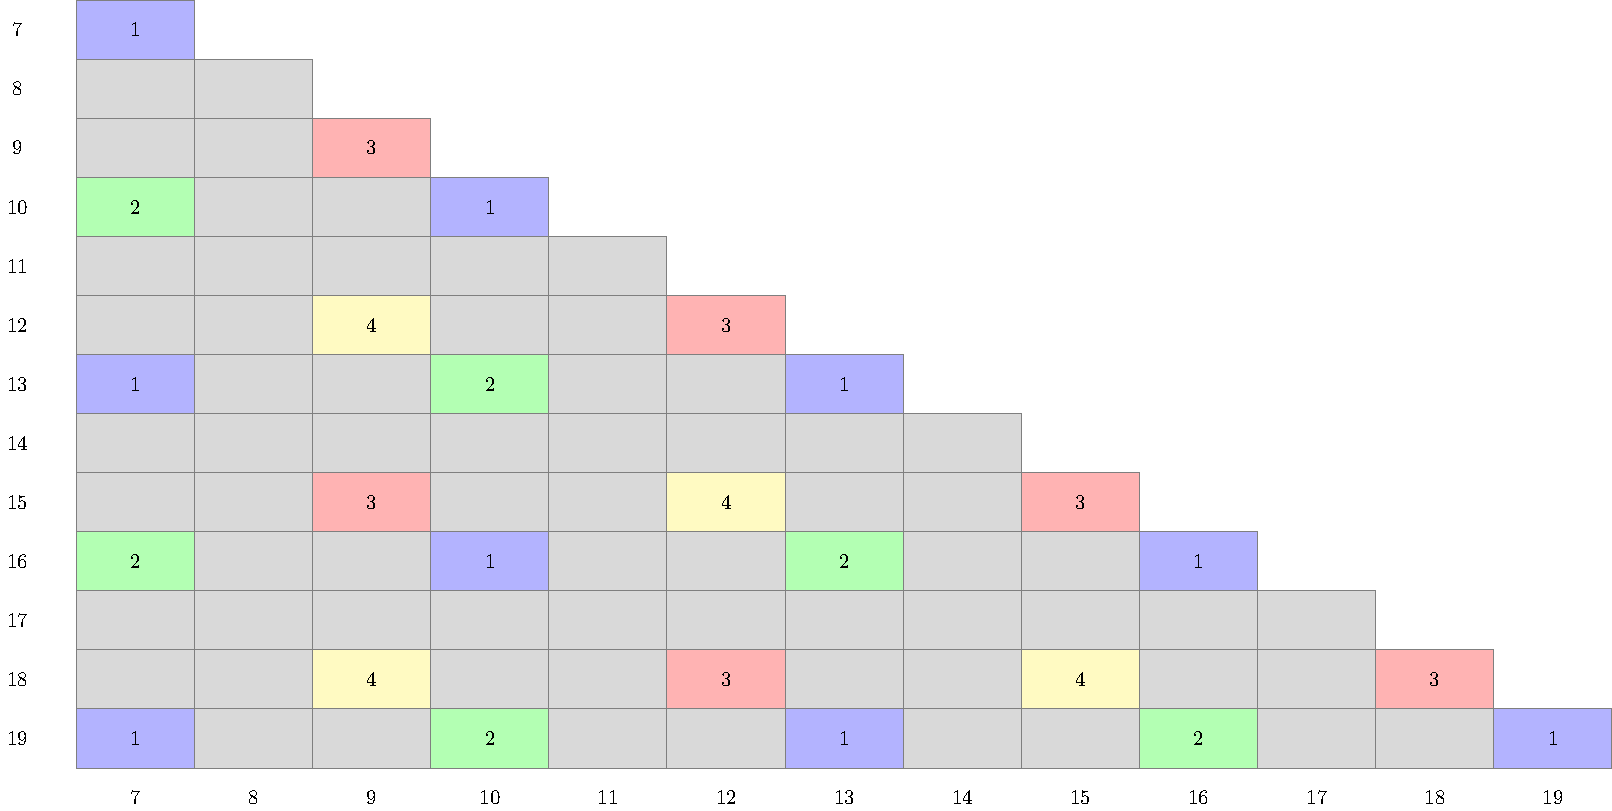
\includegraphics[width=\textwidth]{tables/4/thickness_7_cases.pdf}
\caption{The four thickness 7 cases analyzed in Lemmas \ref{lem:thickness_7_case_1} (blue), \ref{lem:thickness_7_case_2} (green), \ref{lem:thickness_7_case_3} (red), and \ref{lem:thickness_7_case_4} (yellow).}
\label{fig:thickness_7_cases}
\end{table}

\begin{lem}
\label{lem:thickness_7_case_1}
All grids of the form $(x,y,7)$ for $x,y \in \{1,4\}$ and $x \equiv y \pmod 6$ admit perfect lethal sets.
\end{lem}

\begin{proof}
Consider the construction $(a,b,2) + (8,5,5)$ for $a,b \in \{2,5\} \pmod 6$, $a \not\equiv b \pmod 6$, and $a,b > 2$. Observe that this construction obtains all grids of the form described in (1) above, apart from $(10,10,7)$ and $(a, 7,7)$, for $a \equiv 1 \pmod 6$. 

By Corollary \ref{cor:recursion}, we must show that the grids $(a,b,2), (a,5,5), (8,b,5), (8,5,2)$ are all perfect. By Proposition \ref{prop:thickness_2_2d_family}, $(a,b,2)$ and $(8,5,2)$ are perfect. By Lemma \ref{lem:thickness_5_complete}, $(a,5,5)$ and $(8,b,5)$ are perfect. 

To obtain $(a,7,7)$, for $a \equiv 1 \pmod 6$, we consider $(4,4,4) + (a-4,3,3)$. By Corollary \ref{cor:recursion}, we must show that $(4,4,4), (4,3,3), (a-4,4,3), (a-4,3,4)$ are all perfect. We obtain $(4,4,4)$ from $(2,2,2)+(2,2,2)$. By Construction \ref{con:2x2x2} in Appendix A, we have that $(2,2,2)$ is perfect. Proposition \ref{prop:3x3xk} gives $(4,3,3)$. Since $a-4 \equiv 3 \pmod 6$, we obtain $(a-4,4,3)$ from Proposition \ref{prop:thickness_3_width_4}.

To obtain $(10,10,7)$, consider $(5,5,5) + (5,5,2)$. By Corollary \ref{cor:recursion}, we must show that $(5,5,5), (5,5,2), (5,5,2), (5,5,5)$ are all perfect. Lemma \ref{lem:thickness_5_complete} gives us $(5,5,5)$, and Construction \ref{con:5x5x2} gives us $(5,5,2)$. We conclude that all grids of the form given in (1) are perfect. 
\end{proof}

\begin{lem}
\label{lem:thickness_7_case_2}
All grids of the form $(x,y,7)$ for $x,y \in \{1,4\}$ and $x \not\equiv y \pmod 6$ are complete.
\end{lem}

\begin{proof}
Consider the construction $(a,b,2) + (5,5,5)$ for $a,b \in \{2,5\} \pmod 6$, $a \not\equiv b \pmod 6$, and $a,b > 2$. Observe that this construction obtains all grids of the form described in (2) above, apart from $(a,7,7)$, for $a \equiv 4 \pmod 6$. 

By Corollary \ref{cor:recursion}, we must show that the grids $(a,b,2), (a,5,5), (5,b,5), (5,5,2)$ are all perfect. By Proposition \ref{prop:thickness_2_2d_family}, $(a,b,2)$ is perfect. We obtain $(a,5,5)$ and $(5,b,5)$ from Lemma \ref{lem:thickness_5_complete}, and $(5,5,2)$ is given by Construction \ref{con:5x5x2}.

To obtain $(a,7,7)$, for $a \equiv 4 \pmod 6$, we consider $(7,4,4) + (a-7,3,3)$. Since $a \equiv 4 \pmod 6$ and $a \geq 7$, we have that $a \geq 10$. By Corollary \ref{cor:recursion}, we must show that $(7,4,4), (7,3,3), (a-7,4,3), (a-7,3,4)$ are all perfect. We obtain $(7,4,4)$ from $(2,2,2) + (5,2,2)$. Constructions \ref{con:2x2x2} and \ref{con:5x2x2} show that $(2,2,2), (2,2,2), (5,2,2), (5,2,2)$ are all perfect. Proposition \ref{prop:3x3xk} gives us $(7,3,3)$. Since $a-7 \equiv 3 \pmod 6$, we obtain $(a-7,4,3)$ from Proposition \ref{prop:thickness_3_width_4}. We conclude that all grids of the form given in (2) are perfect. 
\end{proof}

\begin{lem}
\label{lem:thickness_7_case_3}
All grids of the form $(x,y,7)$ for $x,y \in \{0,3\}$ and $x \equiv y \pmod 6$ are complete.
\end{lem}

\begin{proof}
Consider the construction $(a,b,2) + (6,9,5)$ for $a,b \in \{0,3\} \pmod 6$, $a \not\equiv b \pmod 6$, and $a,b > 2$. Observe that this construction contains all grids described in (3) above, apart from $(9,9,7)$. 

By Corollary \ref{cor:recursion}, we must show that the grids $(a,b,2), (a,9,5), (6,b,5), (6,9,2)$ are all perfect. By Proposition \ref{prop:thickness_2_2d_family}, $(a,b,2)$ and $(6,9,2)$ are perfect. By Proposition \ref{prop:thickness_3_2d_family}, $(a,9,5)$ is perfect. We obtain $(6,b,5)$ from Lemma \ref{lem:thickness_5_complete}, for $b \geq 5$, and $(6,3,5)$ from Proposition \ref{prop:3x6xk}. 

To obtain $(9,9,7)$, consider $(6,6,4) + (3,3,3)$. By Corollary \ref{cor:recursion}, we must show that $(6,6,4), (6,3,3), (3,6,3), (3,3,4)$ are all perfect. We obtain $(6,6,4)$ from $(3,3,1) + (3,3,3)$. Constructions \ref{con:3x3x1} and \ref{con:3x3x3} show that $(3,3,1), (3,3,3), (3,3,3), (1,3,3)$ are all perfect. Proposition \ref{prop:3x3xk} gives us $(6,3,3)$ and $(4,3,3)$. We conclude that all grids of the form given in (3) are perfect.
\end{proof}

\begin{lem}
\label{lem:thickness_7_case_4}
All grids of the form $(x,y,7)$ for $x,y \in \{0,3\}$ and $x \not\equiv y \pmod 6$ are complete.
\end{lem}

\begin{proof}
Consider the construction $(a,b,2) + (6,6,5)$ for $a,b \in \{0,3\} \pmod 6$, $a \not\equiv b \pmod 6$, and $a,b > 2$. Observe that this construction contains all grids described in (4) above. 

By Corollary \ref{cor:recursion}, we must show that the grids $(a,b,2), (a,6,5), (6,b,5), (6,6,2)$ are all perfect. By Proposition \ref{prop:thickness_2_2d_family}, $(a,b,2)$ is perfect. We obtain $(6,b,5)$ from Lemma \ref{lem:thickness_5_complete}, for $b \geq 5$, and $(6,3,5)$ from Proposition \ref{prop:3x6xk}. We obtain $(6,6,2)$ from $(3,3,1)+(3,3,1)$. By Proposition \ref{prop:purina}, $(3,3,1)$ is perfect, and so by Corollary \ref{cor:recursion}, $(6,6,2)$ is perfect. We conclude that all grids of the form given in (4) are perfect.
\end{proof}

\begin{lem}
Thickness 7 is complete.
\end{lem}

\begin{proof}
By Lemmas \ref{lem:thickness_7_case_1}, \ref{lem:thickness_7_case_2}, \ref{lem:thickness_7_case_3}, and \ref{lem:thickness_7_case_4}, all divisibility cases for thickness 7 admit perfect lethal sets.
\end{proof}

\section{Completeness of Grids of Size $\geq$ 5}

We can get completeness in every residue class modulo 3 by simply considering the grids obtained from $(x,y,z)+(3,3,3)$.

% COMMENT
% COMMENT
% COMMENT
% COMMENT
% COMMENT

\begin{comment}

Let $(a,b,2)$ represent an arbitrary (divisible) grid of thickness 2, and let $x = a \pmod 6$ and $y = b \pmod 6$. By \{some as of yet unwritten construction\}, we have that $(a,b,2)$ percolates at the lower bound for all $x,y \in \{0,2,3,5\}$, where $x \neq y$. We consider two constructions: $(a,b,2) + (6,3,3)$ and $(a,b,2) + (6,6,3)$. 

By item (1) of the remark, in order to show that $(a,b,2) + (6,3,3)$ percolates at the lower bound, it is sufficient to show that $(a,b,2), (a,3,3), (6,b,3), (6,3,2)$ all percolate at the bound. By \{more unwritten constructions\}, this is true for all $x,y \in \{0,2,3,5\}$, where $x \neq y$, $a,b > 1$, and at least one of $\{a,b\} > 2$. (Note that if $a=2$, one of the tuples is $(2,3,3)$, which does not percolate at the lower bound; we accommodate for this by re-writing $(a,b,2) + (6,3,3)$ as $(a,b,2) + (3,6,3)$.) The resulting tuple $(a', b', 5)$ is a grid of thickness 5, with $a'$ and $b'$ in the same residue class modulo $6$, $x,y \geq 8$, and at least one of $\{a',b'\} \geq 9$. From \{some figure representing the divisibility cases of thickness 5\}, we see that the lower bound on $a'$ and $b'$ omits all grids of the form $(5,5,k)$ and $(5,6,k)$, as well as the singular grid $(8,8,5)$. 

Applying an analogous argument to $(a,b,2) + (6,6,3)$, we must demonstrate that $(a,b,2), (a,6,3), (6,b,3), (6,6,2)$ all percolate at the lower bound. By \{some other constructions\}, we again find that this holds for all $x,y \in \{0,2,3,5\}$, where $x \neq y$ and $a,b > 1$. This gives all thickness 5 tuples $(a',b', 5)$ with $a'$ and $b'$ in different residue classes modulo $6$, where $a',b' \geq 8$. 

Combining these results, we have completeness for all grids of thickness 5 except those of the form $(5,5,k)$ and $(5,6,k)$, and the singular grid $(8,8,5)$. By lemmas \ref{lem:width_5} and \ref{lem:width_6}, and \{some construction for $(8,8,5)$\}, these cases are also complete, and so thickness 5 is complete. This completes the proof. 

\end{comment}




